%%%%%%%%%%%%%%%%%%%%%%%%%%%%%%%%%%%%%%%%%%%%%%%%%%%%%%%%%%%%%%%%%%%%%%%%%%%%%%%%
%2345678901234567890123456789012345678901234567890123456789012345678901234567890
%        1         2         3         4         5         6         7         8

\documentclass[letterpaper, 10 pt, conference]{ieeeconf}  % Comment this line out if you need a4paper

%\documentclass[a4paper, 10pt, conference]{ieeeconf}      % Use this line for a4 paper

\IEEEoverridecommandlockouts                              % This command is only needed if 
% you want to use the \thanks command

\overrideIEEEmargins                                      % Needed to meet printer requirements.

%In case you encounter the following error:
%Error 1010 The PDF file may be corrupt (unable to open PDF file) OR
%Error 1000 An error occurred while parsing a contents stream. Unable to analyze the PDF file.
%This is a known problem with pdfLaTeX conversion filter. The file cannot be opened with acrobat reader
%Please use one of the alternatives below to circumvent this error by uncommenting one or the other
%\pdfobjcompresslevel=0
%\pdfminorversion=4

% See the \addtolength command later in the file to balance the column lengths
% on the last page of the document

% The following packages can be found on http:\\www.ctan.org
%\usepackage{graphics} % for pdf, bitmapped graphics files
%\usepackage{epsfig} % for postscript graphics files
%\usepackage{mathptmx} % assumes new font selection scheme installed
%\usepackage{times} % assumes new font selection scheme installed
\usepackage{amsmath} % assumes amsmath package installed
\usepackage{amssymb}  % assumes amsmath package installed
\usepackage{mathtools}
\usepackage{graphicx}
\usepackage{color}
\usepackage{xcolor} % [usenames] (obsolete)
\usepackage{cite}
\usepackage{acronym}
\usepackage{subcaption}
\usepackage{siunitx}
\sisetup{per-mode = symbol}

% \usepackage{soul}
% \usepackage[hyphens]{url}	% this is necessary to allow correct URL line breaks (also at hyphens)
% \renewcommand{\UrlFont}{\small\tt}  % decrease URL font size


\usepackage{tikz}
\usetikzlibrary{
    arrows,
    arrows.meta,
    calc,
    patterns,
}
\usepackage{pgfplots}
\pgfplotsset{compat=newest}

% Comments and debugging:
\newcommand{\DM}[1]{{\color{blue!90!black} \bfseries #1}}
\newcommand{\RS}[1]{\textcolor{red}{#1}}
\newcommand{\FB}[1]{\textcolor{orange}{#1}}
\newcommand{\MS}[1]{\textcolor{magenta}{#1}}

\newcommand{\rads}[0]{\frac{\mathrm{rad}}{\mathrm{s}}}

\acrodef{IMU}{inertial measurement unit}
\acrodef{e-scooter}{electric scooter}

\title{\LARGE \bf On the effects of angular acceleration in orientation estimation using inertial measurement units
}

\author{Felix Brändle, David Meister, Marc Seidel, Robin Strässer, Frank Allgöwer% <-this % stops a space
\thanks{F.\ Allgöwer is thankful that this work was funded by the Ministry of Science, Research and the Arts of the State of Baden-Württemberg (MWK) in the context of the ``MobiLab'' Project.
F.\ Brändle thanks the International Max Planck Research School for Intelligent Systems (IMPRS-IS) for its support.
D.\ Meister, M.\ Seidel, R.\ Strässer thank the Graduate Academy of the SC SimTech for its support.}% <-this % stops a space
\thanks{F.\ Brändle, D.\ Meister, M.\ Seidel, R.\ Strässer, and F.\ Allgöwer are with the University of Stuttgart, Institute for Systems Theory and Automatic Control, 70550 Stuttgart, Germany
(e-mail: e-scooter@ist.uni-stuttgart.de).}%
}

%===============================================================================
\begin{document}
\maketitle
\thispagestyle{empty}
\pagestyle{empty}


%%%%%%%%%%%%%%%%%%%%%%%%%%%%%%%%%%%%%%%%%%%%%%%%%%%%%%%%%%%%%%%%%%%%%%%%%%%%%%%%
\begin{abstract}
    Determining the orientation of a rigid body using an \acl{IMU} is a common problem in many engineering applications.
    However, sensor fusion algorithms suffer from performance loss when other motions besides the gravitational acceleration affect the accelerometer.
    In this paper, we show that linear accelerations caused by rotational accelerations lead to additional zeros in the linearized transfer functions, which are strongly dependent on the operating point.
    These zeros lead to non-minimum phase systems, which are known to be challenging to control.
    In addition, we demonstrate how Mahony and Madgwick filters can mitigate the effects of the additional acceleration, but at the cost of reduced bandwidth.
    This generates insights into a fundamental problem in estimation, that are transferable to many practical applications.
\end{abstract}
 
\section{Introduction} \label{sec:intro}

To achieve true scalability on massive datasets, a modern query engine
needs to be able to take advantage of large, shared-memory, multicore
systems.  Cloud companies offer servers with dozens of cores and many
terabytes of main memory; for example systems with up to 224 physical
cores and 24TB of main memory are available on
AWS~\cite{aws-ec2-high-memory}.  Users who need to perform complex
data analytics on large datasets will likely use such large servers
for their needs, and expect the query engine to scale up.  The
research community has studied parallel algorithms for query
processing extensively for over three decades, initially with a focus
on shared-nothing
architectures~\cite{DBLP:journals/tkde/DeWittGSBHR90,DBLP:journals/sigmod/DeWittG90,DBLP:journals/cacm/DeWittG92,DBLP:conf/vldb/DeWittNSS92},
but also on the shared-memory, multicore architectures that are the
focus of this
paper~\cite{DBLP:journals/vldb/BonczK99,DBLP:conf/sigmod/BlanasLP11,DBLP:conf/sigmod/ZhangHZH19,DBLP:conf/sigmod/ShahvaraniJ20,DBLP:conf/sigmod/0001MHGZHMM21,DBLP:conf/sigmod/0001MHGZHMM21,DBLP:conf/sigmod/WuWZ22}.
Many modern database engines use multi-threads during query
evaluation, and thus are prepared to use multiple cores, when they are
available.

{\em Binary joins} are conceptually easy to parallelize on a multicore
system: both relations are hash-partitioned, then the join is computed
in parallel in each partition.  Practical challenges consist of
reducing the number of blocking steps, reducing the number of cache
misses, and reducing the overhead of locks.  There exist several
solutions for these challenges, see for example the excellent
discussion in~\cite{DBLP:conf/sigmod/BlanasLP11}.

However, applications like graph databases, social network analysis, 
RDF/Sparql engines, queries on knowledge graphs, and even sparse tensor
compilers, are using a different approach to compute multi-join
queries, called \emph{Worst-Case Optimal Join},
WCOJ~\cite{DBLP:conf/icdt/Veldhuizen14,DBLP:conf/spire/BrisaboaCFN15,DBLP:conf/sigmod/ChuBS15,DBLP:conf/sigmod/AbergerTOR16,DBLP:journals/pvldb/FreitagBSKN20,DBLP:conf/sigmod/ArroyueloHNRRS21,DBLP:journals/pacmmod/WangWS23,DBLP:journals/sigmod/Salihoglu23,DBLP:conf/cidr/JinFCLS23}.
The WCOJ algorithms are theoretically optimal, and are known to
outperform binary joins on cyclic queries (but not on acyclic ones),
making them well-suited for these specialized engines and even for
some general-purpose relational
engines~\cite{DBLP:conf/sigmod/ArefCGKOPVW15,DBLP:journals/pvldb/FreitagBSKN20}.

Unfortunately, there is no obvious adaptation of a parallel 
hash-partitioned binary join to WCOJ.  Unlike a traditional query plan, a WCOJ
algorithm joins all relations at once.  The algorithm consists of
several nested loops, with one iteration for each join variable of the
query.  There exist a few parallel implementations of WCOJ, and they
parallelize only the topmost loop.  For example both
LogicBlox~\cite{DBLP:conf/sigmod/ArefCGKOPVW15} and
Umbra~\cite{DBLP:journals/pvldb/FreitagBSKN20} \revB{, as well as its Diamond-hardened extension~\cite{DBLP:journals/pvldb/BirlerKN24},} adopt this simple
parallelization strategy.  Under this approach, the system
hash-partitions the domain of the topmost variable into sets of equal
size, then executes the query for each partition in a separate logical
thread.  Each thread executes the remaining loops of the WCOJ
sequentially.  As a consequence, while each thread reads only a small
fragment of the relations that contain the first iteration variable,
it reads and processes the other relations entirely.  In other words,
relations that do not contain the top-most variable are not
partitioned at all under this approach.

\begin{figure*}[t]
  \setlistingalphabet
  \begin{minipage}[t]{.31\textwidth}
    
    
    
    \begin{lstlisting}[caption={Original Query}, style=BashInputStyle,
    lineskip=0pt,
    abovecaptionskip=0pt,
    label=lst:serial]
Q := R(X,Y), S(Y,Z), T(Z,X)

For x $\in$ !\colorbox{yellow}{R.X $\cap$ T.X}!
  For y $\in$ !\colorbox{green}{R[x].Y $\cap$ S.Y}!
    For z $\in$ !\colorbox{pink}{S[y].Z $\cap$ T[x].Z}!
      Q += (x, y, z)
\end{lstlisting}
   
  \end{minipage}
  \hfill
  \begin{minipage}[t]{.34\textwidth}
    \begin{lstlisting}[caption={Traditional Parallelization}, style=BashInputStyle,
    lineskip=-1pt,
    abovecaptionskip=0pt,
    label=lst:tradpara]  
// Parititon R.X and T.X on X
// In parallel,  Thread i:
For x $\in$ !\colorbox{yellow}{R\tssr{i}.X $\cap$ T\tssr{i}.X}!
  For y $\in$ !\colorbox{green}{R\tssr{i}[x].Y $\cap$ S.Y}!
    For z $\in$ !\colorbox{pink}{S[y].Z $\cap$ T\tssr{i}[x].Z}!
      Q += (x, y, z)
    \end{lstlisting}
    
  \end{minipage}
  \hfill
  \begin{minipage}[t]{.34\textwidth}
    \begin{lstlisting}[caption={\name's Parallelization}, style=BashInputStyle,
    lineskip=-1pt,
    abovecaptionskip=0pt,
    label=lst:newpara]  
// Partition R, S and T (see text)
// In parallel, Thread (i, j, k) 
For x $\in$ !\colorbox{yellow}{R\tssr{ij}.X $\cap$ T\tssr{ik}.X}!
  For y $\in$ !\colorbox{green}{R\tssr{ij}[x].Y $\cap$ S\tssr{jk}.Y}!
    For z $\in$ !\colorbox{pink}{S\tssr{jk}[y].Z $\cap$ T\tssr{ik}[x].Z}!
      Q += (x, y, z)
    \end{lstlisting}
    
  \end{minipage}

  
  
\caption{Comparison of WCOJ Parallelization Algorithms}
\label{fig:algo-comp}
  
  

\setlistingnumbering
\end{figure*}

In this paper, we introduce \name, a parallel version of WCOJ,
optimized for large multicore, shared-memory systems.  \name
partitions the domain of every variable, not just the top-most
variable, and creates a separate thread for every combination of
partitions.  This idea has been originally proposed for shared-nothing
architectures, first for MapReduce
systems~\cite{DBLP:conf/edbt/AfratiU10}, then was studied extensively
under a theoretical model of computation called Massively Parallel
Communication (MPC) model, where the algorithm is known as the {\em HyperCube Algorithm}~\cite{DBLP:journals/jacm/BeameKS17,DBLP:conf/icdt/KoutrisBS16,DBLP:journals/ftdb/KoutrisSS18,DBLP:journals/sigmod/HuY20,DBLP:conf/pods/Hu21}.

\revB{\name overcomes three limitations of the traditional WCOJ
  parallelization method: load skew, work duplication, and contention
  due to lazy index creation.  We start by illustrating the first
  limitation of the traditional method, load skew, using an example.}

\eat{
one
important limitation of the traditional parallelization approach:

the skew in the load of the threads.  We illustrate that with an
example.}

\begin{figure}[htbp]
  \centering
  \includegraphics[width=.75\linewidth]{skew}
  \caption[Skewness for Triangle Query on WGPB]{ \revB{Skewness for Triangle Query on WGPB. Here each of the three lines 
  
  represents the same number of partitions, $4096$, but allocated differently to the three attributes $X$, $Y$, and $Z$. The expression $4096 \times 1 \times 1$ (the blue line) means that the attribute $X$ was partitioned into $4096$ buckets and assigned to the threads, while the attributes $Y$, $Z$ were not partitioned (or partitioned into $1$ bucket). Similarly, $16 \times 16 \times 16$ (the orange line) means that each of $X$, $Y$, $Z$ was partitioned into $16$ buckets, for a total of $4096$ buckets/threads. Each point in the graph represents the runtime of one of the $4096$ threads, run in isolation, on one core; when executed on all $60$ cores, these threads will be dynamically scheduled on all $60$ cores, using work stealing.}}
  \label{fig:skew-eg}
\end{figure}

\begin{example} \label{ex:intro:1} Listing~\ref{lst:serial} in
  Fig.~\ref{fig:algo-comp} illustrates WCOJ with the triangle query
  $Q(X,Y,Z) = R(X,Y), S(Y,Z), T(Z,X)$.  We ran this query on the
  (undirected) WGPB~\cite{wgpb-dataset, DBLP:conf/semweb/HoganRRS19} dataset, with $54.0$M nodes and $81.4$M edges,
  using 4096 threads on a server with 60 physical cores and 120
  hyperthreads.\footnote{As we will see in Sec.~\ref{sec:exp}, \name keeps all cores busy, making hyperthreading ineffective, thus the ideal speedup is only a factor of 60, not 120.}  The traditional
  way to parallelize this query is shown in
  Listing~\ref{lst:tradpara}.  The domain of the first variable, $X$,
  is partitioned into 4096 fragments.  This partitions $R(X,Y)$ and
  $T(Z,X)$, but does not partition $S(Y,Z)$.  Each thread
  $i=1,2,\ldots,4096$ reads only a $1/4096$-fragment of $R$ and $T$,
  but reads the entire relation $S$.  We instrumented the code to
  measure, for each thread, its runtime:\footnote{In examples, we focus only on the join runtime,  given preprocessing is complete.} we show their distribution as
  the blue line in Fig.~\ref{fig:skew-eg}.  The skew (ratio between
  the largest and smallest runtime) is quite visible, showing a factor
  of more than 15. \revC{The cumulative time of the 4096 threads, i.e. the area under
  the curve, is 308s.  We used standard work-stealing to execute the
  threads on the 60 cores, thus, in an ideal scenario the total
  runtime should be $308/60 = 5.13$s: however, the actual measured
  total runtime (shown in the table at the top left) was 13.83s.
  As we will see, the discrepancy is mostly due to skew.}
  
  
\end{example}

Instead of the traditional parallelization technique, \name partitions
all query variables.

We illustrate this with an
example.

\begin{example} \label{ex:intro:2} Listing~\ref{lst:newpara} in
  Fig.~\ref{fig:algo-comp} shows how \name executes the triangle
  query, by partitioning each variable domain.  On the MPC model, the
  theoretically optimal partitioning is $16\times 16\times 16$,
  meaning that the domain of each variable $X, Y, Z$ is
  hash-partitioned into 16 buckets.  A thread is identified by a
  triple $(i,j,k)$, where each of $i,j,k$ range from $1$ to $16$, and
  it will only read a fragment of $1/16^2 = 1/256$ of each relation
  $R, S, T$.  The runtime distribution is the orange line in
  Fig.~\ref{fig:skew-eg}. \revC{The total work performed by the 4096
    threads (area under the curve) was $300$s, almost identical to the
    traditional method (Example~\ref{ex:intro:1}).  But} the skew
  ratio is only about 4, and the actual measured runtime on 60 cores
  decreased to 6.57s.  \revC{By reducing the load skew, \name reduced
    runtime by $2\times$.}

\end{example}

\revC{The second limitation of the traditional approach is work
  duplication.  For example, referring to Listing~\ref{lst:tradpara},
  the fragment $S[y]$ of the relation $S$ needs to be accessed by all
  4096 threads in order to perform the intersection
  $S[y].Z \cap T_i[x].Z$.  In order to reduce or to eliminate
  redundant work, \name departs from the theoretical MPC model,
  because the optimal partitioning strategy of the MPC model may also
  lead to work duplication. For example, in Listing~\ref{lst:newpara},
  the fragment $R_{ij}[x]$ of the relation $R$ needs to be accessed by
  all 16 threads $k=1,2,\ldots,16$ in order to perform the
  intersection $R_{ij}[x].Y \cap S_{jk}.Y$.}

\revB{One contribution in \name is a novel cost-based optimization of
  the number of buckets allocated to each variable, called the {\em
    share} of that variable.

  While the problem of computing optimal shares has been extensively
  studied by the MPC model, their solutions do not carry over to
  multicores.  The reason is that in the MPC model the communication
  is separated from the computation, and the optimal shares minimize
  only the communication cost, ignoring any work duplication at the
  servers.  In a shared-memory system there is no communication cost,
  instead the total work becomes the main cost.  \name computes the
  optimal shares using a cost model, which aims to minimize both skew
  and work duplication.}

\begin{example}
  The problem in the previous example is that, by partitioning the
  last variable $Z$, we create duplicated work for intersections of
  the previous variables.  Two threads with identifiers $(i,j,k_1)$
  and $(i,j,k_2)$ will see exactly the same partition $R_{ij}$.  In
  addition, if the data is dense, then they will likely also see
  similar values in $T_{ik}.X$, $S_{jk}.Y$. This causes portions of
  the top loops to be executed redundantly by different threads.  The
  choice of how many shares to allocate for each variable depends on
  the data distribution.  In our example, \name choose as optimal
  shares $64 \times64 \times 1$.  \revC{The load distribution for
    these shares is the green line in Fig.~\ref{fig:skew-eg}, and the
    cumulative load of all 4096 threads (area under the curve) has
    decreased to $114$s, from about $300$s for the
    $4096 \times 1 \times 1$ and the $16 \times 16 \times 16$ shares.
    As a consequence, the actual measured runtime on 60 cores
    decreased to $2.46$s.}
    

\end{example}

We introduced a novel cost model specifically for shared-memory,
parallel WCOJ, based on a pessimistic cardinality
estimator~\cite{DBLP:conf/sigmod/CaiBS19}, more precisely on a recent
refinement~\cite{DBLP:journals/pacmmod/KhamisNOS24} that uses more
sophisticated statistics on the input relations rather than just their
cardinalities.  To the best of our knowledge this is the first cost
model proposed for WCOJ.\footnote{Recent
  work~\cite{DBLP:journals/pvldb/WangT0O23} circumvents the need for a
  cost model for WCOJ by using Reinforcement Learning for choosing the
  variable order.}  Our cost model is described in
Sec.~\ref{subsec:cost:model}.

\revB{Finally, the third limitation of the traditional approach comes
  a particular optimization in modern WCOJ systems, the lazy
  construction of the hash-trie, which in the parallel setting leads
  to contention between threads.}

All WCOJ implementations index the data, in order to speed up the
intersections that need to be done at each iteration of the algorithm.
While a standard trie was used in an early implementation of
WCOJ~\cite{DBLP:conf/icdt/Veldhuizen14}, recent implementations use a
hash trie index.  For each relation, the first level of the trie is a
hash table consisting of values of the first variable, pointing to
hash tables consisting of values of the second variable, and so on.
Since the hash trie construction is expensive, recent systems compute
lazily the entries on levels two and higher: only sub-tries that are
actually needed are
constructed~\cite{DBLP:journals/pvldb/FreitagBSKN20,DBLP:journals/pacmmod/WangWS23}.
We illustrate this in Fig.~\ref{fig:hashtrie}, where the lazy sub-trie
construction applies to $R.Z$ and $T.Z$.  However, when done in
parallel, the lazy index requires all index accesses to be coordinated
via locks, in order to avoid read-write conflicts.  This is not a
problem for a small number of cores, say 12-16, but it becomes a
problem for a larger number of cores, which is our target for \name.

To avoid this contention and further remove the need for locks, \name
introduces a new, and simple sort-based trie index that we call
Compressed Column layout, or \indexlayout.  Level $k$ of \indexlayout
is a sorted array, consisting of the first $k$ attributes of the
relation, which pointers to the next level of the trie.  We construct
\indexlayout eagerly, by first sorting the entire relation once, then
computing each level by a projection and duplication elimination.  We
benefit from the fact that there exists very effective parallel,
shared-memory sorting algorithm: \name uses \textbf{ips4o} (In-place
Parallel Super Scalar Samplesort)~\cite{axtmann2017,
  axtmann2020engineering} for this purpose.  By replacing the
hash-based index with a sort-based one we reduce the construction time
significantly, and this allows us to compute it eagerly, and avoiding
any need for coordination during the parallel execution of
WCOJ. \revB{Thus, \indexlayout represents a return to the original
  trie in LFTJ~\cite{DBLP:conf/icdt/Veldhuizen14}, but in a simplified
  form, where the entire level $k$ is a single array, which allows us
  to construct the entire index using a single parallel sort.}

Finally, a last challenge of the WCOJ algorithm that we observed in
\name is that it some duplicated work can be avoided by storing
intermediate results and using them later.  Each loop of a WCOJ
computes the intersection of all domains of the current variable.
Some of these intersections are computed repeatedly, for different
iterations of some outer loop.  This occurs in both sequential and
parallel implementations of WCOJ, but it seems to impact more the
parallel implementation.  To address that, we introduce an
optimization that we call a \emph{rewriting mechanism}.  We precompute
this intersection during the outer loop, then take advantage of the
shared memory that allows multiple threads to read that intermediate
result.  We describe the rewriting mechanism in
Sec.~\ref{subsec:rewrite}.

We have evaluated our methods and compared them with the state-of-the-art
parallel implementations of WCOJ. Our approach, \name, demonstrates
strong scalability, achieving near-linear scaling observed up to 60 cores.
\name outperforms other baselines by 3x on the WGPB dataset, which
consists of sparse and skewed data, and can be 10x to 100x faster than
competing systems on dense data.  We report our evaluation in
Sec.~\ref{sec:exp}.

In summary, we make the following contributions: 

\begin{itemize}
\item We describe \name, a parallel version of WCOJ that adapts the
  HyperCube algorithm to a multicore system (Sec.~\ref{sec:join}).
\item We present a novel trie structure index \indexlayout that faciliates and accelerates the operations of WCOJ (Sec.~\ref{sec:prep}).
\item We introduce a rewriting mechanism that further reduces redundant
  computation of the parallel WCOJ (Sec.~\ref{subsec:rewrite}).
\item We propose a new cost model for the parallel WCOJ and use it for
  computing an optimal partition share allocation (Sec.~\ref{subsec:cost:model} and Sec.~\ref{subsec:plan}).
\item We conduct an extensive experimental evaluation
  (Sec.~\ref{sec:exp}).
\end{itemize}


 %\input{sec2-mathematical-derivation}
% !TEX root=root.tex
% ##############################################################################################
% MODEL
% ##############################################################################################
\section{MODEL}\label{sec:Model}
To model the effects of angular motion around a fixed axis on the estimation, we consider a pendulum as illustrated in Fig.~\ref{IMG:Setup:Pendulum}.
The pendulum generalizes many types of rotational motions, which are not centered around the rotational axis, e.g., loops in aerobatics, joint motions in exoskeletons, or curve driving in vehicles \cite{Nazarahari2021, Gajamohan2012}, such that our results can be easily transferred to different setups.
The \ac{IMU} is placed at a fixed distance $l$ to the point $O$ and rotates with respect to the roll angle $\varphi$ while pitch $\theta$ and yaw $\psi$ are held at zero.
Hence, any acceleration in $\varphi$ causes a linear acceleration that can be measured by the accelerometer of the \ac{IMU}.

We align the rotation of the pendulum with the roll angle to investigate whether an acceleration in $\varphi$ influences the pitch and yaw estimation.
Note that the same analysis can be performed around an arbitrary axis, except for the yaw component, which cannot be estimated using accelerometers.
Reconstruction of the yaw angle requires additional sensors, e.g., a magnetometer, which also provides redundancy for estimating the pitch angle~\cite{Madgwick2011}. 
An investigation including magnetometers is beyond the scope of this paper and is left for future research.
The \ac{IMU} is able to measure the linear acceleration $a^K$ including gravity and the angular velocity $\omega^K$, both expressed in the body fixed coordinate system $K$, which is rotated with respect to the inertial frame $I$. 
This results in the measurement equations
\begin{equation}
	a^K = \begin{pmatrix}
		0 \\
		\sin(\varphi) - \frac{l}{g}\ddot{\varphi} \\
		\cos(\varphi) - \frac{l}{g}\dot{\varphi}^2
	\end{pmatrix} 
	,\qquad 
	\omega^K = \begin{pmatrix}
		\dot{\varphi}\\ 
		0 \\
		0
	\end{pmatrix}.
\end{equation}
These acceleration measurements are already expressed in units of standard gravity [$g$] and we assume that $\varphi$ is twice differentiable to ensure the existence of $\ddot{\varphi}$.
Since the acceleration depends only on the ratio of $l$ and $g$, we normalize $g$ to 1 in the following. 
Further, a common assumption in literature is that the \ac{IMU} is at rest, i.e., $\dot{\varphi}=\ddot{\varphi}=0$ such that only gravity affects $a^K$~\cite{Madgwick2011, Mahony2008, Ludwig2018a}.
Hence, it is possible to compute $\varphi$ by applying a simple trigonometric function to $a^K$.
In the remainder of the paper, we analyze the effects when the \ac{IMU} is not at rest.
\begin{figure}[tb]
	\centering
	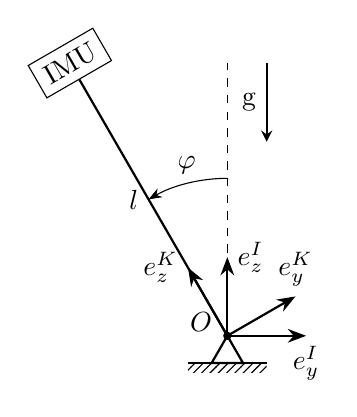
\begin{tikzpicture}[scale=1]
	
	\def\varphiang{-30}
	\def\height{4}
	\def\rArc{0.5*\height}
	
	\def\groundlength{1}
	\def\groundheight_plot{0.12}
	
	\def\supportLength{0.4}
	
	\coordinate (origin) at (0,0);
	\coordinate (originKOS) at ($(origin)$); %-(0.5*\groundlength,0)$);
	\coordinate (IMU) at ($(origin) + ({\height*sin(\varphiang)},{\height*cos(\varphiang)})$);
	
	% Pendulum
	\draw[thick] (origin) -- (IMU) node[midway,left] {$l$};
	
	\draw[dashed](origin) --++ ($({0},{\height*cos(\varphiang)})$);
	
	\draw[-Stealth] ($(origin) + ({0},{\rArc})$) arc(90:90-\varphiang:\rArc) node[midway, above]{$\varphi$};
	
	% IMU
	\node[draw,fill = white, rotate = -\varphiang] at (IMU) {IMU};
	
	% Coordinate System
	\draw[-Stealth,thick] (originKOS) --++ (1,0) node[below]{$e_y^I$};
	\draw[-Stealth,thick] (originKOS) --++ (0,1) node[right]{$e_z^I$};
	
	\draw[-Stealth,thick] (originKOS) --++ ($({cos(\varphiang)},{-sin(\varphiang)})$) node[above]{$e_y^K$};
	\draw[-Stealth,thick] (originKOS) --++ ($({sin(\varphiang)},{cos(\varphiang)})$) node[left]{$e_z^K$};
	
	\fill (origin) circle(1.5pt) node[yshift = -2, xshift = -2, above left]{$O$};
	
	% Ground
	
	
	\coordinate (groundStart) at ($(origin)-(0,{\supportLength*sin(60)})-({0.5*\groundlength},0)$);	
	
	\fill[pattern=north east lines] (groundStart) rectangle ++(\groundlength,-\groundheight_plot);	
	\draw[thick] (groundStart) -- ++(\groundlength,0);	
	
	% Support
	\draw[thick] (origin) --++ ($({\supportLength*cos(60)}, {-\supportLength*sin(60)})$) --++ ($(-\supportLength,0)$) -- (origin);
	
	% Gravity
	\draw[thick,-stealth] ($(origin)+({0.5*\groundlength},{\height*cos(\varphiang)})$) --++(0,-1) node[midway, left]{$\mathrm{g}$};
	
\end{tikzpicture}

	\caption{Pendulum with \acs{IMU} including gravity g.}
	\label{IMG:Setup:Pendulum}
\end{figure}

\input{sec3-analysis}
\input{sec4-experiment}
\input{sec5-outlook}

% Bibliography
\bibliographystyle{IEEEtran}
\bibliography{CCTAScooterIMU}
                                                   

\end{document}
